\documentclass[runningheads]{llncs}
%\pagestyle{plain}
%usepackage
%\usepackage[demo]{graphicx}
\usepackage{subfig}
\usepackage{tabularx}
\usepackage{array,multirow,graphicx}
\usepackage{float}

\usepackage{cite}
\usepackage{amssymb}
\usepackage{amsmath}
\usepackage{amsfonts}
\usepackage{amscd}
\usepackage{enumerate}
\usepackage{url}
\usepackage{algorithm, algorithmic}
%\usepackage[a4paper,left=2.5cm,right=2cm,top=1.8cm,bottom=1.8cm]{geometry}
\usepackage{upquote}
\usepackage{multicol}

\usepackage{slashbox}  % create diagonal line in tables

%\usepackage{hyperref}
%\usepackage[nameinlink]{cleveref}
%\usepackage{tikz}
%\usepackage{mdframed}
%\usepackage{textcomp}


\renewcommand{\algorithmicrequire}{\normalsize \textbf{Input:}}
\renewcommand{\algorithmicensure}{\normalsize \textbf{Output:}}
\renewcommand{\algorithmicwhile}{\normalsize \textbf{while}}

 \renewcommand\UrlFont{\color{blue}\rmfamily}
%def
\def\N{\mathbb{N}}
\def\Z{\mathbb{Z}}
\def\Q{\mathbb{Q}}
\def\R{\mathbb{R}}
\def\C{\mathbb{C}}
\def\F{\mathbb{F}}


\usepackage{color}
\usepackage{listings} 
\usepackage{xspace}  % to allow for text macros that don't eat space 
\usepackage[misc,geometry]{ifsym}


\lstdefinelanguage{Sage}[]{Python}
{morekeywords={True,False,sage,singular},
	sensitive=true}
\lstset{frame=none,
	showtabs=False,
	showspaces=False,
	showstringspaces=False,
	commentstyle={\ttfamily\color{dredcolor}},
	keywordstyle={\ttfamily\color{dbluecolor}\bfseries},
	stringstyle ={\ttfamily\color{dgraycolor}\bfseries},
	language = Sage,
	basicstyle={\small \ttfamily},
	aboveskip=.3em,
	belowskip=.1em
}
\definecolor{dblackcolor}{rgb}{0.0,0.0,0.0}
\definecolor{dbluecolor}{rgb}{.01,.02,0.7}
\definecolor{dredcolor}{rgb}{0.8,0,0}
\definecolor{dgraycolor}{rgb}{0.30,0.3,0.30}
\newcommand{\dblue}{\color{dbluecolor}\bf}
\newcommand{\dred}{\color{dredcolor}\bf}
\newcommand{\dblack}{\color{dblackcolor}\bf}

\renewcommand{\emph}[1]{{\dblack{#1}}}

\newcommand{\Sage}{{\color{dbluecolor}\sf Sage}\xspace}



\newcommand{\keywords}[1]{\par\addvspace\baselineskip
	\noindent\keywordname\enspace\ignorespaces#1}


\begin{document}
\title{Solving LWR via BDD Strategy:\\
Modulus Switching Approach}

\author{Huy Quoc Le\inst{1}$^\textrm{(\Letter)}$, Pradeep Kumar Mishra\inst{1},  Dung Hoang Duong\inst{2}, \\ Masaya Yasuda\inst{3, 4}}

\authorrunning{H. Q. Le et al.}
\institute{
Graduate School of Mathematics, Kyushu University,\\
744 Motooka, Nishi-ku, Fukuoka-shi, Fukuoka-ken, 819-0395, Japan.
\\
\email{q-le@math.kyushu-u.ac.jp}\\
\email{p-mishra@math.kyushu-u.ac.jp}\\
\and 
School of Computing and Information Technology, University of Wollongong,\\
Northfields Avenue, Wollongong NSW 2522, Australia.\\
\email{hduong@uow.edu.au}
\and
Institute of Mathematics for Industry, Kyushu University, \\
744 Motooka, Nishi-ku, Fukuoka-shi, Fukuoka-ken, 819-0395, Japan.\\
\and 
JST, CREST,\\
4-1-8 Honcho, Kawaguchi, Saitama, 332-0012, Japan.\\
\email{yasuda@imi.kyushu-u.ac.jp}}
\maketitle

\medskip

\begin{abstract}
	%Recently, the Learning with Rounding (LWR) problem has been used in constructing many lattice-based cryptosystems among which some were submitted to the NIST competition for post-quantum cryptography. For cryptanalysis, t
The typical approach in attacking an LWR$_{m,n,q,p}(\chi_s)$ instance parameterized by four integers $m$, $ n$, $q$, $p$ $ (q \geq p)$ and a probability distribution $\chi_s$ is just by simply regarding it as a Learning with Errors (LWE) modulo $q$ instance and then trying to adapt known LWE attacks to this LWE instance. In this paper, we show that for an LWR$_{m,n,q,p}(\chi_s)$ instance whose parameters satisfy a certain sufficient condition, one can use the BDD strategy to recover the secret with higher advantages if one transforms the LWR instance to an LWE modulo $q'$ instance with $q'$ chosen appropriately instead of an LWE modulo $q$ instance.  The optimal modulus $q'$ used in our BDD attack is quite close to $p$ as well as typically smaller than $q$. Especially, our experiments confirm that our BDD attack is much better in solving search-LWR in terms of root Hermite factor, success probability and even running time either in case the ratio $\log (q)/ \log (p)$ is big or/and the dimension $n$ is sufficiently large.

\keywords{Learning with Errors (LWE) $\cdot$ Learning with Rounding (LWR) $\cdot$ Bounded Distance Decoding (BDD) strategy $\cdot$ Modulus switching $\cdot$ Lattice basis reduction $\cdot$  Babai's Nearest Plane (BNP) algorithm.}
\end{abstract}


%===============
\section{Introduction}
%===============

The LWR problem introduced by Banerjee, Peikert and Rosen in \cite{BPR12} is a de-randomization variant of the well-known LWE problem in which a $(q,p)$-modulo rounding function (denoted by $\lfloor \cdot \rceil_{q,p}$) is used to hide the secret instead of using an error $e$ drawn from some distribution. 
Specifically, for $x \in \mathbb{Z}_q$ we have $\lfloor x \rceil_{q,p}=\left \lfloor (p/q) \cdot x \right \rceil \in \mathbb{Z}_p$, where $\lfloor x \rceil$ rounds the real number $x$ to the nearest integer. Let $n \geq 1$, $q \geq p \geq 2$, and given a secret vector $\mathbf{s} \in \mathbb{Z}_q^n$, an LWR sample is the pair $(\mathbf{a},c) \in \mathbb{Z}_q^n \times \mathbb{Z}_p$, in which the vector $\mathbf{a} \leftarrow \mathbb{Z}_q^n$ uniformly at random and $c:=\lfloor\langle \mathbf{a},\mathbf{s} \rangle \rceil_{q,p}\in \mathbb{Z}_p$. 


%LWR problem has many applications in lattice-based cryptography such as pseudorandom functions \cite{BPR12}, lossy trapdoor functions, reusable extractors \cite{AKPW13}, key homomorphic PRFs \cite{BLMR13}, signature scheme \cite{HPWZ17}, etc. Also 

Several LWR-based cryptosystems have recently been submitted to NIST for Post-Quantum Cryptography Standardization, for instance Round2 \cite{BBGM+17} and  Lizard \cite{CKLS16}. In their proposals, for efficiency goal, the secret is sampled from (even sparse) small sets. For example, in  \cite{CKLS16}, the authors consider the binary secrets $\{0,1\}^*$ or trinary secrets $\{-1,0,1\}^*$ or even the secret $\mathbf{s}$ is sampled from some uniform distribution over $\{-1,0,1\}^*$ in which $\mathbf{s}$ contains $h$ nonzeros for some fixed integer $h>0$. 

%There are some analyses of hardness of the LWR problem based on reducing LWR to LWE under certain constrains on parameters such as \cite{BPR12},  \cite{AKPW13}, \cite{BGM+15}, \cite{AA16}. Their reductions are independent of the distribution from which the secret is drawn. 

A typical approach in attacking LWR is to transfom an LWR instance to an LWE modulo $q$. More specifically, the following method, called \textit{$q$-reduction}, is used to lift an LWR instance
$(\mathbf{a}, c=\left\lfloor \langle \mathbf{a}, \mathbf{s} \right \rangle \rceil_{q,p}) \in \mathbb{Z}_q^{n} \times \mathbb{Z}_p$ to an LWE instance modulo $q$ of the form $(\mathbf{a},c'=\langle \mathbf{a},\mathbf{s} \rangle+e) \in \mathbb{Z}_q^{n} \times \mathbb{Z}_q$, where
$c'=\left \lfloor \frac{q}{p}c \right \rceil $ and 
 $e \in \left( -\frac{q}{2p},\frac{q}{2p} \right]$. 
 Most of techniques for solving LWR are adapted from attacks against an LWE modulo $q$ instance  \cite{BBGM+17, CKLS16, DTV15} such as SIS strategy, BDD strategy, uSVP strategy, algebraic strategy \cite{AG11} and so on (cf. \cite{APS15} for more details). In this work, we just focus on the BDD strategy which aims to reduce a search-LWE instance to the closest vector problem (CVP),  then use a practical lattice basis reduction algorithm (such as Lenstra-Lenstra-Lov\'{a}sz (LLL) algorithm \cite{LLL82} or the blockwise Korkine-Zolotarev (BKZ) algorithm \cite{SE94}) along with the Babai's Nearest Plane (BNP) algorithm \cite{Bab86} to solve this CVP instance.

Some questions can be raised here that if it is possible to transform an LWR$_{m,n,q,p}(\chi_s)$ instance to an LWE instance modulo $q'$ (called \textit{$q'$-approach}) other than an LWE modulo $q$ (called \textit{$q$-approach}), with $q'<q$ or even $q'>q$, that if the $q'$-approach is better for specific attacks (such as the BDD strategy  we are going to focus on) than the $q$-approach and that if so, how to choose the optimal $q'$. Note that, in the case of $q'<q$, the transformation is the so-called \textit{modulus switching} technique. The technique allows to transform an LWE modulo $q$ instance to an LWE modulo $q'$ instance with $q'$ is typically chosen as
\begin{equation}\label{keye}
 q' \approx \frac{\sigma_s}{\sigma}\cdot \sqrt{\frac{n}{12}}\cdot q,
\end{equation} 
where $n$ is the length of the secret and $\sigma_{s}$,  $\sigma$ are standard deviations of the secret and the error of the original LWE mod $q$ instance, respectively (cf. \cite[Lemma 2]{APS15} for more details). 
The modulus switching technique was used for the first time aiming to speed up the homomorphic encryption operations \cite{BV11a}. Then the technique was also used to evaluate the classical  hardness of LWE problem \cite{BLP+13}. Recently, the technique was modified to combine with BKW algorithm on LWE \cite{AFFP14}. Until now, however, the effect of the technique on other attacks against LWE and LWR has not been studied carefully.

\subsubsection{Our contribution.} We evaluate the impact of modulus switching on the BDD strategy in solving search LWR problem. We achieved the following:
\begin{enumerate}
	\item We reduce an LWR$_{m,n,q,p}(\chi_s)$ instance to an LWE modulo $q$ instance and obtain an induced error $e$.  Some previous works stated that the error \textit{heuristically} follows a uniform distribution over $[-q/2p, q/2p)$ (see, e.g., \cite[Sec. 4.2.1]{CKLS16}) then its variance is roughly $\frac{q^2}{12p^2}$. We will confirm that the error actually  follows a discrete uniform distribution and hence we compute its variance that is more precisely equal to $\frac{q^2+2pq}{12p^2}$, which is much larger than $\frac{q^2}{12p^2}$ if $q\gg p$. This helps us to estimate $q'$ (mentioned below) more exactly than previous works. 

\item We also determine the successful range in which LWR instances can be solved by the BDD strategy using practical lattice reduction algorithms (e.g., LLL or BKZ) accompanied with the BNP algorithm \cite{Bab86}.

\item We theoretically and experimentally convince that one can transform an LWR$_{m,n,q,p}(\chi_s)$ instance to an LWE modulo $q'\approx \sqrt{\frac{(m-n)(n\sigma_s^2+1)p^2q^2}{n(q^2+2q)}}$ which can be solved more ``efficiently" by the BDD strategy under a sufficient condition. By ``efficiently", we mean that we will have either higher success probability and smaller root Hermite factor or/and smaller running time in solving this LWE instance depending on how much the size of $\alpha$  is. Our approach is especially suitable for LWR instances with short secret, i.e., $\sigma_s$ small.

\end{enumerate}

Our main technical tool is a heuristic evaluation on the success probability of the BDD strategy. To the best of our knowledge, this work is the first attempt to evaluate carefully the modulus switching's effect to the BDD strategy on LWR problem. We expect that our work will provide with a different perspective in exploiting modulus switching technique not only to solve LWR (even LWE) (by the BDD strategy or even other strategies) but also in other application scenarios.
%If $A=\{a_i \in \mathbb{R}|1\leq i \leq m\}$ and $k\in \mathbb{R}$ then $kA=\{k\cdot a_i \in \mathbb{R}|1\leq i \leq m\}$. 
\subsubsection{Notation.}If $A=\{a_1, \cdots ,a_m\}$ with $a_i\in \mathbb{R}$ then $k\cdot A=\{k\cdot  a_1,\cdots,k\cdot  a_m\}$ for any $k\in \mathbb{R}$. The logarithm of base 2 (resp., the natural logarithm) of a positive real number $x$ will be written as $\log (x)$ (resp., $\ln(x)$). We use $\mathcal{U}(A)$ to indicate the uniform distribution over the set $A$. The rounding operation $\lfloor a \rceil$ outputs the integer closest to $a$ and in the case of a tie, it outputs the integer next to $a$. For any positive integer $q$, we denote by $\mathbb{Z}_q=\{0,1, \cdots, q-1\}$ the set of integers modulo $q$. We write $x \leftarrow \chi$ to say that the random variable $x$ follows the probability distribution $\chi$ or $x$ is sampled from the distribution $\chi$. For a real number $k$, the notation $y \leftarrow k \cdot \chi$ means that $y=k \cdot x$ for some $x$ that follows the probability distribution $\chi$.


%==============================
\section{Preliminaries}
%==============================


%=======================
\subsection{Lattices}
%=======================

%Let $\mathbf{a}_1,\cdots,\mathbf{a}_{m}$ be $m$ linearly independent vectors in $\mathbb{Z}^n$. 
The lattice $\mathcal{L}=\mathcal{L}(\mathbf{A})$ generated by the column matrix $\mathbf{A}=[\mathbf{a}_1,\cdots,\mathbf{a}_{m} ] \in \mathbb{Z}^{n \times m}$ of $m$ linearly independent vectors is defined to be the set of all linear integral combinations of $\mathbf{a}_{i}$'s, i.e., 
	$\mathcal{L}(\mathbf{A})=\left\{ \mathbf{A}.\mathbf{x}: \mathbf{x} \in \mathbb{Z}^{m}\right\}=\left\{ \sum_{i=1}^{m} x_i\mathbf{a}_i: x_i \in \mathbb{Z}\right\}.  $
We call the matrix $\mathbf{A}$ \textit{a basis} of $\mathcal{L}$ and call each $\mathbf{a}_i$ \textit{a basis vector}. The rank of the lattice is the number of basis vector (i.e., $m$). The dimension of the lattice is the number of entries in each basis vector (i.e., $n$). If $m=n$, the lattice is called to be \textit{full-rank}. Note that, every lattice has infinitely many bases up to a unimodular matrix of determinant $\pm1$. Hence, if $\mathbf{A}$ and $\mathbf{B}$ are two different bases of the lattice $\mathcal{L}$, then $\det (\mathbf{A}^T \mathbf{A})=\det (\mathbf{B}^T \mathbf{B})$. We call $\det(\mathcal{L}(\mathbf{A})):=\sqrt{\det (\mathbf{A}^T \mathbf{A})}$ the \textit{determinant} (or \textit{volume}) of the lattice $\mathcal{L(\mathbf{A})}.$ 

\textit{The Gram-Schmidt} matrix $\mathbf{A}^{*}=\{\mathbf{a}^{*}_1,\cdots,\mathbf{a}^{*}_{m} \}$ for a basis $\mathbf{A}=\{\mathbf{a}_1,\cdots,\mathbf{a}_{m} \}$ is defined by setting
$\mathbf{a}^{*}_1=\mathbf{a}_1\text{ and } \mathbf{a}^{*}_{i}=\mathbf{a}_{i}-\sum_{j=1}^{i-1} \frac{\langle \mathbf{a}_{i}, \mathbf{a}^{*}_j \rangle}{\Vert\mathbf{a}^{*}_j\Vert^2},  i=2,\cdots,m.$ Note that $\det(\mathcal{L}{(\mathbf{A})})=\prod_{i=1}^{m}\Vert \mathbf{a}_i^* \Vert.$
The \textit{fundamental parallelepiped} asscociated with a basis $\mathbf{A}=\{\mathbf{a}_1,\cdots,\mathbf{a}_{m}\}$ is $\mathcal{P}_{1/2}(\mathbf{A})=\left\{ \sum_{i=1}^{m} x_i\mathbf{a}_i: x_i \in \left[-\frac{1}{2},\frac{1}{2} \right)\right\}. $ We define the fundamental parallelepiped $\mathcal{P}_{1/2}(\mathbf{A}^{*})$ for the Gram-Schmidt matrix $\mathbf{A}^{*}$ in the same way.


For integers $q, m, n$ $(m \geq n)$, given a random matrix $\mathbf{A} \in \mathbb{Z}_q^{m \times n}$, we consider the so-called $q$-\textit{ary lattice}
$\Lambda_q{(\mathbf{A})}=\left\{ \mathbf{u} \in \mathbb{Z}^m: \mathbf{u}=\mathbf{A}\mathbf{s} \text{ mod } q \text{ for some } \mathbf{s} \in \mathbb{Z}^n \right\}.$
It is well known that $\text{det}(\Lambda_q(\mathbf{A})) = q^{m-n}$ with high probability.
%=======================
\subsection{Lattice Basis Reduction Algorithms and Root Hermite Factor} \label{sec2.2}
%=======================
A basis of a lattice can be reduced using the so-called \textit{lattice basis reduction} (LBR) algorithms to obtain a new basis consisting of short and nearly orthogonal lattice vectors. Such two algorithms typically used in practice are LLL \cite{LLL82} and BKZ \cite{SE94}. The former is a polynomial-time algorithm and the latter is a block version of the former with exponential complexity.

Let $\mathcal{L}$ be a lattice of rank $m$ and $\mathbf{A}$ be a reduced lattice basis obtained using some LBR algorithm, say $\mathcal{A} $, the \textit{root Hermite factor} (rHF) $\delta_{\mathcal{A}}$ of $\mathcal{A} $ with respect to $\mathbf{A} $ is the constant given by
\begin{equation}\label{keyk}
\delta_{\mathcal{A} }=\left( \frac{||\mathbf{u}_1||}{\det(\mathcal{L})^{1/m}} \right)^{\frac{1}{m}},
\end{equation}
where $\mathbf{u}_1$ is the shortest non-zero vector of $\mathbf{A} $. 
Gama and Nguyen in \cite{GM08} attempted to estimate the rHF of LLL and BKZ for random matrices. Namely, they estimated that the rHF of LLL is $\delta_{\text{LLL}}\approx 1.0219$ on average in high dimension $\geq 100$ while  that of BKZ with blocksize $\beta=20$ \footnote[1]{BKZ of blocksize $20$ is usually used in practice because of its time/quality trade-off property.} is $\delta_{\text{BKZ}}\approx 1.0128$.

Unfortunately, however, these experimental results of \cite{GM08} for random matrices may be not perfectly fit for $q$-ary lattices. That is the reason why Kudo et al. in \cite{KYGY16} conducted intensively an experiment on $q$-ary lattices to estimate the quantity $\min_{i=1}^{m}\Vert \mathbf{b}_i^* \Vert$ from which they defined an alternative measure as follows:
\begin{equation}\label{eq1}
c_{\mathcal{A}}:=\left( \frac{\min_{i=1}^{m}\Vert \mathbf{b}_i^* \Vert}{\det(\Lambda_q{(\mathbf{A})})^{1/m}}\right)^{\frac{1}{m}},
\end{equation}
where $\mathbf{b}_i^*$'s are Gram-Schmidt vectors of a basis of the $q$-ary lattice $\Lambda_q{(\mathbf{A})}$, say $\mathbf{B}=\{ \mathbf{b}_1,\cdots,\mathbf{b}_{m}\}$, that is already reduced by some LBR algorithm $\mathcal{A} $. Note that $c_{\mathcal{A}} \leq 1$ since $\min_{i=1}^{m}\Vert \mathbf{b}_i^* \Vert \leq (\prod_{i=1}^{m}\Vert \mathbf{b}_i^* \Vert)^{1/m} =\det(\Lambda_q{(\mathbf{A})})^{1/m} $. Especially, Kudo et al. \cite{KYGY16} estimated that
	$c_{\text{LLL}}=0.9775$
	whereas using BKZ with blocksize $\beta=20$, they got 
	$c_{\text{BKZ}}=0.9868$ (cf. \cite[Table 1]{KYGY16}).

If we still denote the rHF for $q$-ary lattices by $\delta_{\mathcal{A}}$ then it seems that $\delta_{\mathcal{A}} \approx 1/c_{\mathcal{A}}$. For instance, with $c_{\text{LLL}}=0.9775$ and $c_{\text{BKZ}}=0.9868$, we have $1/c_{\text{LLL}}=1.0230$ and $1/c_{\text{BKZ}}=1.0139$, respectively, that are quite close to the rHF for random matrices mentioned above.

We will use \eqref{eq1} to reach an important heuristic that is useful for our work (see Subsection \ref{heu}).

%=======================
\subsection{Probability}
%=======================

%=======================
 \subsubsection{Variance of Random Variables.}
 %=======================
 We denote the variance of a random variable $X$ by $\sigma_X$.
  For $a, b \in \mathbb{Z}$, the variance of a random variable $X$ following the discrete uniform distribution $\mathcal{U}(\{a, a+1,\cdots, b-1,b\})$ is 
	$\sigma_{X}^2=((b-a+1)^2-1)/12$. 
	If $X$ follows the continuous uniform distribution $\mathcal{U}(a,b)$ then
	$\sigma_{X}^2=(b-a)^2/12.$ Assuming that $Z=X+Y$ where $X,Y $ are independent random variables then $\sigma^2_Z=\sigma^2_X+\sigma^2_Y.$ Finally, for every random variable $X$ and for every constant $k\in \mathbb{R}$, let $Y=kX$, then we have
	$\sigma^2_Y=k^2\sigma^2_{X}$.
	


\subsubsection{Gaussian Distribution.} For any real numbers $\mu, x \in \mathbb{R} $ and any real number $s>0$, the one dimensional continuous Gaussian distribution $\mathcal{D}_{\mu, \sigma}$ of mean $\mu$ and variance $\sigma^2$ is defined by its probability density function (pdf)
$\mathcal{D}_{\mu, \sigma}(x)=\frac{1}{\sqrt{2\pi \sigma^2}} \cdot e^{-\frac{(x-\mu)^2}{2\sigma^2}}, \forall x \in \mathbb{R}.$
\subsubsection{Convolution of Two Distributions.} Let $X$ and $Y$ be continuously distributed independent random variables with pdfs $f_X$ and $f_Y$. Then the pdf of the random variable $Z=X+Y$ is the convolution of $f_X$ and $f_Y$ given by
\begin{equation}\label{keycon}
f_Z(z)=(f_X*f_Y)(z)=\int_{-\infty}^{+\infty}f_X(t)f_Y(z-t)dt=\int_{-\infty}^{+\infty}f_X(z-t)f_Y(t)dt.
\end{equation}

%=======================
\subsection{ Search-LWE and BDD Strategy}  \label{heu}
%=======================

LWE problem proposed in \cite{Reg09} has been playing important role in lattice-based cryptography. The hardness of most of the lattice-based cryptosystems is based on the LWE problem which has two versions: one is decision version and another is search version. Here, we recall the search version of the LWE problem.
%=======================
\begin{definition}[Search-LWE Problem]
%=======================
 Given positive integers $n, q$, a fixed secret vector $\mathbf{s}$ whose each component is sampled from some distribution $ \chi_s$ and another probability distribution $\chi_e$ on $ \mathbb{Z}$, the search-LWE$_{m,n,q,\chi_s, \chi_e}$ problem is to find the secret $\mathbf{s}$ from $m$ LWE samples of the form $(\mathbf{a},c=\langle \mathbf{a}, \mathbf{s}\rangle +e \text{ mod } q) \in  \mathbb{Z}_q^n \times  \mathbb{Z}_q,$ where $\mathbf{a} \in \mathbb{Z}_q^n$ is drawn uniformly at random, and the error term $e \leftarrow \chi_e$.
 \end{definition}
	
	If we have such $m$ samples $(\mathbf{a}_i,c_i=\langle \mathbf{a}, \mathbf{s}\rangle +e_i)$ for $i=1,\cdots,m$, we can collect them as  $(\mathbf{A},\mathbf{c}=\mathbf{A}.\mathbf{s}+\mathbf{e})$ in which $\mathbf{A}$ is an $(m \times n)$- matrix whose $i$-th row is $\mathbf{a}_i$, $\mathbf{c}=(c_1,c_2,\cdots,c_m)^T$, and $\mathbf{e}=(e_1,e_2,\cdots,e_m)^T$.
	
%=======================
\subsubsection{BDD Strategy.} 
%=======================
The BDD strategy for solving search-LWE proposed by Lindner and Peikert \cite{LP11} is based on the close relation between search-LWE problem and BDD problem. Given a lattice and a target vector unusually close to the lattice, BDD problem asks to find the lattice vector closest to the target. 

Let $(\mathbf{A}, \mathbf{c}=\mathbf{A}\mathbf{s}+\mathbf{e} \mod q) \in \mathbb{Z}_q^{m \times n} \times \mathbb{Z}_q^m$  be a search-LWE$_{m,n,q,\chi_s, \chi_e}$ instance. Also let $\Lambda_q{(\mathbf{A})}=\left\{ \mathbf{u} \in \mathbb{Z}^m: \mathbf{u}=\mathbf{A}\mathbf{s} \text{ mod } q \text{ for some } \mathbf{s} \in \mathbb{Z}^n \right\}$ be  the $q$-ary lattice spanned by columns of $\mathbf{A}$ and we call it \textit{the associated $q$-ary lattice} of the search-LWE problem $(\mathbf{A}, \mathbf{c})$. To solve search-LWE problem via the BDD strategy, we reduce it to a CVP. In fact, if the error $\mathbf{e}$ is sufficiently short then $\mathbf{c}$ is closest to some lattice point $\mathbf{u}=\mathbf{A}\mathbf{s} \text{ mod } q \in \Lambda_q(\mathbf{A})$ since we have $\mathbf{e}=\mathbf{c}-\mathbf{A}\mathbf{s}.$  Thus, finding the secret $\mathbf{s}$ is equivalent to finding $\mathbf{u}$, i.e., solving a CVP problem over $q$-ary lattice $\Lambda_q{(\mathbf{A})}$.

The most basic tools used in solving search-LWE via BDD strategy are some basis reduction algorithm, say $\mathcal{A}$ (e.g., LLL or BKZ), and the BNP algorithm. The BNP algorithm takes as input the vector  $\mathbf{c}$  and a basis $\mathbf{B}=\{ \mathbf{b}_1,\cdots,\mathbf{b}_{m}\}$ of  $\Lambda_q(\mathbf{A})$ that is already reduced by $\mathcal{A}$. Finally, the BNP algorithm outputs the lattice point $\mathbf{u} \in \Lambda_q(\mathbf{A})$ such that $\mathbf{e}=\mathbf{c}-\mathbf{u} \in\mathcal{P}_{1/2}(\mathbf{B^*}) $. 

From now on, by ``BDD strategy" or ``BDD attack", we mean the BDD strategy associated with the BNP algorithm. 

%=======================
\paragraph{Success Probability of  the BDD Strategy.} 
%=======================
The success probability of the BDD strategy in solving search-LWE is measured by the probability of the event that the error $\mathbf{e}$ lies in $\mathcal{P}_{1/2}(\mathbf{B^*})$.
Depending on which distribution the error $\mathbf{e}$ follows, we have some formulas to compute the probability in literature: (i) if $\mathbf{e}$ is uniform then we can estimate the probability by
 \begin{equation}\label{eq18}
  \mathrm{Pr}\left[ \mathbf{e} \in \mathcal{P}_{1/2}(\mathbf{B^*})\right]= \prod_{i=1}^{m}\left(  \frac{ \rceil \Vert\mathbf{b}^{*}_i \Vert}{2\sigma_e\sqrt{3}} \right), 
 \end{equation}
(ii) in the case of a Gaussian error $\mathbf{e}$, we can use the formula taken from \cite{LP11}
 \begin{equation}\label{eqkk}
 \mathrm{Pr}\left[ \mathbf{e} \in \mathcal{P}_{1/2}(\mathbf{B^*})\right]=\prod_{i=1}^{m}\mathrm{erf}\left( \frac{ \rceil \Vert \mathbf{b^{*}}_i \Vert}{2 \sigma_e \sqrt{2}} \right),
 \end{equation} 
 where $\sigma^2_e $ is the variance of the error $\mathbf{e}$ according to its distribution and $\mathrm{erf}(\cdot)$ is the Gaussian error function 
 $\mathrm{erf}(z)=\frac{2}{\sqrt{\pi}}\int_{0}^{z} \text{exp}(-t^2)dt, z \in [0, +\infty].$
However, \eqref{eq18} and \eqref{eqkk} are really not helpful for our work \footnote[2]{We cannot use either \eqref{eq18} or \eqref{eqkk} if the error $\mathbf{e}$ has a complex behavior. Such a kind of error is the $q'$-error that we will see in Section \ref{sec5}.}. Therefore, we have to look for another way to estimate the success probability for the BDD strategy regardless of the error's distribution. Fortunately, we can use a heuristic analysis appeared in \cite{KYGY16} as follows:

We have $\mathrm{Pr}\left[ \mathbf{e} \in \mathcal{P}_{1/2}(\mathbf{B^*})\right]=\mathrm{Pr}\left[\vert \langle \mathbf{e}, \mathbf{b}_i^{*} \rangle \vert < \Vert \mathbf{b}_i^{*} \Vert^2/2, \forall i=1,...,m\right].$ Using the heuristics
$\vert \langle \mathbf{e}, \mathbf{b}_i^{*} \rangle \vert  \approx \Vert \mathbf{e} \Vert \cdot \Vert \mathbf{b}_i^{*} \Vert /\sqrt{m}$ and  $\Vert \mathbf{e} \Vert \approx \sigma_e \cdot \sqrt{m}$, we have  $2 \sigma_e \leq \Vert \mathbf{b}_i^{*} \Vert \text{ for all } i=1,...,m,$ which is equivalent to 
\begin{equation}\label{keym}
2 \sigma_e \leq \min_{i=1,...,m}\Vert \mathbf{b}_i^* \Vert.
\end{equation}
Combining \eqref{keym} with \eqref{eq1} yields the following heuristic that will be very useful for our work:
%=======================
\subsubsection{Heuristic 1.} 
%=======================
\textit{Let $c_{\mathcal{A}}$ is defined as in \eqref{eq1}. Heuristically, the success probability for the BDD strategy in solving search-LWE problem $(\mathbf{A}, \mathbf{c}=\mathbf{A}\mathbf{s}+\mathbf{e} \mod q) \in \mathbb{Z}_q^{m \times n} \times \mathbb{Z}_q^m$ can be measured by the probability
%\begin{equation*} \label{eeq3}
$\mathrm{Pr}\left[2\sigma_e \leq c_{\mathcal{A}}^m \cdot \det(\Lambda_q{(\mathbf{A})})^{1/m}\right],$
%\end{equation*}
namely,
%\begin{equation} \label{eq3}
$\mathrm{Pr}\left[2\sigma_e \leq c_{\mathcal{A}}^m \cdot q^{(m-n)/m}\right]$
%\end{equation}
which is equivalent to
\begin{equation}\label{eqa}
\mathrm{Pr} \left[\frac{q^{m-n}}{\sigma_e^m} \geq  \frac{2^m}{c_{\mathcal{A}}^{m^2}}\right],
\end{equation}
where $\mathcal{A}$ is the LBR algorithm used within the BDD strategy.}

\paragraph{BDD Strategy and Root Hermite Factor.} It is conventional that the quality of the reduced basis (which is characterized by the rHF obtained using by some LBR algorithm) has the most significant effect on the success probability of the BNP algorithm (see, e.g., \cite[Section 5.4]{APS15}, \cite{BBD+15, GvVW17}), hence the BDD strategy. Namely, smaller rHF means that the corresponding basis is reduced better, hence the BNP algorithm may return the closest vector more precisely, so the efficacy of the BDD strategy may be higher.  

Assume the BDD strategy uses the LBR algorithm named $\mathcal{A}$.  And suppose that we want to compare the efficacy of the BDD strategy in solving a search-LWE problem $(\mathbf{A}_1, \mathbf{c}_1)$ with that in solving a search-LWE problem  $(\mathbf{A}_2, \mathbf{c}_2)$. Then instead of success probability, we can compare the rHFs of $\mathcal{A}$ with respect to the reduced bases of the associated $q$-ary lattices $\Lambda_q{(\mathbf{A}_1)}$ and $\Lambda_q{(\mathbf{A}_2)}$.
%=======================
\subsection{Search LWR and a Reduction from LWR to LWE}
%=======================

Let $ p, q $ be two moduli such that $2 \leq p \leq q $. Recall that, the $(q,p)$-modulo rounding operation, denoted by $\lfloor. \rceil_{q,p}$, is defined as follows: for $x \in \mathbb{Z}_q$ $\lfloor x \rceil_{q,p}=\lfloor (p/q)\cdot x \rceil \in \mathbb{Z}_p$. We can extend the operation for vectors, matrices by taking it component-wise, such as for $\mathbf{x}=(x_{1},\cdots, x_{n}) \in \mathbb{Z}_q^n$, we have
$\lfloor \mathbf{x} \rceil_{q,p}=( \lfloor x_{1} \rceil_{q,p},\cdots,\lfloor x_{n} \rceil_{q,p}).$

%=======================
\begin{definition}[LWR Sample]
	%=======================
 For a secret vector $\mathbf{s} \leftarrow \chi_s$ where $\chi_s$ is some distribution of variance $\sigma^2_s$, an LWR$_{m,n,q,p}(\chi_s)$ sample is obtained by choosing a vector $\mathbf{a} \leftarrow \mathbb{Z}_q^n$ uniformly at random and outputting $(\mathbf{a},c=\lfloor\langle \mathbf{a},\mathbf{s} \rangle \rceil_{q,p})\in \mathbb{Z}_q^n \times \mathbb{Z}_p$.
\end{definition}
Assuming that we have such $m$ LWR samples then we can write them as $(\mathbf{A},\mathbf{c}=\lfloor \mathbf{A}\mathbf{s}  \rceil_{q,p}) \in \mathbb{Z}_q^{m \times n} \times \mathbb{Z}_p^m$, where $\mathbf{A}$ is a matrix whose rows are $\mathbf{a}_i$ and $\mathbf{c}$ is a column vector whose elements are $c_i$.

%=======================
\begin{definition}[Search-LWR] 
%=======================
Given $m$ LWR samples  $(\mathbf{A},\mathbf{c}=\lfloor \mathbf{A}\mathbf{s}  \rceil_{q,p}) \in \mathbb{Z}_q^{m \times n} \times \mathbb{Z}_p^m$, the search-LWR$_{m,n,p,q}(\chi_s)$ problem is to find the secret $\mathbf{s}$.
\end{definition}

%=======================
\subsubsection{Reducing LWR$_{m,n,q,p}(\chi_s)$ to LWE Modulo $q$.} 
%=======================

The following reduction, called \textit{$q$-reduction}, is used to transform an LWR instance consisting of samples of the form
$(\mathbf{a}, c=\left\lfloor \langle \mathbf{a}, \mathbf{s} \right \rangle \rceil_{q,p}) \in \mathbb{Z}_q^{n} \times \mathbb{Z}_p$ to an LWE modulo $q$ instance of the form $(\mathbf{a},c_1) \in \mathbb{Z}_q^{n} \times \mathbb{Z}_q$ in which
\begin{equation} \label{eq4}
\begin{split}
c_1&=\left \lfloor \frac{q}{p} \cdot c \right \rceil \text{mod } q\\
&=\left \lfloor \frac{q}{p}.\left(\frac{p}{q} \cdot (\langle \mathbf{a}, \mathbf{s} \rangle+qu) +e_1 \right)\right\rceil \text{mod } q, \text{with } e_1 \in \left( -\frac{1}{2},\frac{1}{2} \right], u \in \mathbb{Z}, \\
&=(\langle \mathbf{a}, \mathbf{s} \rangle +e)\text{ mod } q=\langle \mathbf{a}, \mathbf{s} \rangle \text{ mod } q+e, \text{ where } e:=\left \lfloor (q/p) \cdot e_1 \right \rceil.\\
\end{split}	
\end{equation}
For short, we call the error $e$ \textit{$q$-error}.
%=======================

Note that, in the reduction above, we used the following assumption:
\subsubsection{Assumption 1.} \textit{We assume that in our work, the error induced by reduction from an LWR instance to a corresponding LWE instance is not changed by a modulo operation. 
Formally, for an LWE sample} $(\mathbf{a},(\langle \mathbf{a}, \mathbf{s} \rangle +e)\text{ mod } q) \in \mathbb{Z}_q^{n} \times \mathbb{Z}_q$, \textit{we assume that} $$(\langle \mathbf{a}, \mathbf{s} \rangle +e)\text{ mod } q=\langle \mathbf{a}, \mathbf{s} \rangle \text{ mod } q+e.$$
This assumption was also used in many previous works relating to LWE such as \cite{BGV12, BV11a,BV11b,KYGY16, LL15}. We still use this assumption in Section \ref{sec5}.
%=======================
%=======================
\section{Distribution of the $q$-Error}\label{sec3}
%=======================

	The $q$-reduction above has been typically considered in recent works relating to the LWR problem (see, e.g., \cite{BBGM+17,CKLS16, FLX+16}).  In these works, it is heuristically assumed that $e$ is continuously uniform over $\left( -{q}/(2p),{q}/(2p) \right]$. If so, the variance is just $\sigma^2 \approx {q^2}/{(12p^2)}$. In this section, we show that $ e $ is actually distributed according to a discrete uniform distribution over the set $\left\{ -\left\lfloor{\lfloor q/2 \rfloor}/{p} \right \rceil, \cdots, \left\lfloor {\lfloor q/2 \rfloor}/{p} \right \rceil \right\}$, hence its variance is actually $\sigma^2\approx (q^2+2pq)/(12p^2)$ which is significantly greater than $q^2/(12p^2)$ in the case $q \gg p$.
	
	
	To begin with, we state a simple lemma on rounding operation via discrete uniform distribution.
	%=======================
	\begin{lemma}\label{lem1}
	%=======================
	Given a nonzero real number $b$. Set $b_0:=-\lfloor b \rceil$, $b_1:=-\lfloor b \rceil+1$, $\cdots,b_{t-1}:=\lfloor b \rceil-1$ and $b_t:= \lfloor b \rceil $ and  define the set $B:=\{b_0, \cdots, b_t\}$. Let $x$ be a real number taken uniformly at random from $[-b, b]$. Then
		\begin{equation*}\label{eq5}
		\mathrm{Pr}[\lfloor x \rceil=b_i| b_i \in B]=\mathrm{Pr}[\lfloor x \rceil=b_j| b_j \in B], \text{ for all } i,j \in \{1,...,t-1\}.
			\end{equation*}
In particular,
			\begin{equation*}\label{eq6}
		\mathrm{Pr}[\lfloor x \rceil=b_0]=\mathrm{Pr}[\lfloor x \rceil=b_t]\leq \mathrm{Pr}[\lfloor x \rceil=b_i| b_i\in B], \forall i \in \{1,...,t-1\}.
			\end{equation*}
	\end{lemma}	

\proof {The idea for the proof is easy. Firstly, note that, for $1 \leq i \leq t-1$, we have
		$$\mathrm{Pr}[\lfloor x \rceil=b_i]=\mathrm{Pr}[x \in [b_i-1/2, b_i+1/2)],$$
which implies the first statement in the lemma.
Secondly, since $b_0=-\lfloor b \rceil$ and $b_t=\lfloor b \rceil$, so $b_0-1/2 \leq -b < b_0+1/2$ and $b_t-1/2 \leq b < b_t+1/2$,
$$\mathrm{Pr}[\lfloor x \rceil=b_0]=\mathrm{Pr}[x \in [-b, b_0+1/2)] \leq \mathrm{Pr}[x \in [b_0-1/2, b_0+1/2)],$$
and $$\mathrm{Pr}[\lfloor x \rceil=b_t]=\mathrm{Pr}[x \in [b_t-1/2, b]] \leq \mathrm{Pr}[x \in \left[b_t-1/2, b_t+1/2 \right)].$$} \qed 
	Now we give the theorem describing the behavior of $q$-error $e$.
	
%=======================
	\begin{theorem}
%=======================
	Set $b:=\frac{\lfloor q/2 \rfloor}{p}$ and $A:=\left\{ -\left\lfloor b \right \rceil+1, \cdots, \left\lfloor b \right \rceil -1 \right\}$. Also let $e$ be the $q$-error defined as in \eqref{eq4}. Then we have:
		$$ \mathrm{Pr}[e=a|a \in A]= \frac{1}{2b}, \text{ and } \mathrm{Pr}[e=-\left\lfloor b \right \rceil]=\mathrm{Pr}[e=\left\lfloor b \right \rceil]= \frac{b-\left \lfloor b\right \rceil +\frac{1}{2}}{2b}\leq \frac{1}{2b}.$$
		However, less precisely, we can say that $e$ is uniform over $$B:=\left\{-\left\lfloor b \right \rceil,  -\left\lfloor b \right \rceil+1, \cdots, \left\lfloor b \right \rceil -1, \left\lfloor b \right \rceil \right \}.$$
		Then the variance of $q$-error $e$ is
		\begin{equation}\label{key}
		\sigma^2 \approx \frac{\left (2\left \lfloor \frac{\lfloor q/2 \rfloor}{p} \right \rceil +1 \right)^2-1}{12} \approx \frac{q^2+2qp}{12p^2}.
		\end{equation} 
	\end{theorem}
	\proof 
	
		First, we show that the error $e_1$ appears in \eqref{eq4} is distributed uniformly over $\frac{1}{q} \cdot \left\{-\lfloor q/2 \rfloor, \cdots, \lfloor q/2 \rfloor \right\}$. 
	Note that, we fix the secret $\mathbf{s}$ which is sampled from some probability distribution $\chi_s$ beforehand. It is true that if we take $\mathbf{a} \in \mathbb{Z}_q^{n}$ uniformly at random then ($\left \langle\mathbf{a}, \mathbf{s} \right\rangle \text{mod }q$) is also uniform over $\mathbb{Z}_q$. Hence, $\frac{p}{q} \cdot (\left \langle\mathbf{a}, \mathbf{s} \right\rangle \text{mod }q)$ is also uniform over $\frac{p}{q} \cdot \mathbb{Z}_q=\{0,p/q,\cdots, p \cdot (q-1)/q\}$. 
	Suppose that $\left \langle\mathbf{a}, \mathbf{s} \right\rangle \text{mod }q=k$, for some $k\leftarrow \mathcal{U}(\{0,\cdots,q-1\})$. There always exist integers $w$ and $v$ such that  $kp=qw+v$, $-\lfloor q/2 \rfloor \leq v \leq \lfloor q/2 \rfloor$, and $ 0 \leq w \leq p$. Certainly, $v$ is uniform over the set $\{-\lfloor q/2 \rfloor ,\cdots,\lfloor q/2 \rfloor \}$. Thus, $(p/q)\cdot (\left \langle\mathbf{a}, \mathbf{s} \right\rangle \text{mod }q)=kp/q=w+v/q$, where $-\lfloor q/2 \rfloor/q \leq v/q \leq  \lfloor q/2 \rfloor/q$.
	Consequently, $\left \lfloor (p/q) \cdot (\left \langle\mathbf{a}, \mathbf{s} \right\rangle \text{mod }q) \right\rceil =w \in \{0,\cdots,p\}$, and hence $$e_1:=\frac{p}{q}(\left \langle\mathbf{a}, \mathbf{s} \right\rangle \text{mod }q)-\left \lfloor \frac{p}{q}(\left \langle\mathbf{a}, \mathbf{s} \right\rangle \text{mod }q) \right\rceil =\frac{v}{q}$$ is uniform over $(1/q) \cdot \{-\lfloor q/2 \rfloor ,\cdots,\lfloor q/2 \rfloor \}$. As a result, $(q/p) \cdot e_1=v/p$ is uniform over $\{-{\lfloor q/2 \rfloor}/p, \cdots, {\lfloor q/2 \rfloor}/p\}.$ 
	
	Recall that, the $q$-error $e=\left \lfloor (q/p) \cdot e_1 \right \rceil.$ Applying Lemma \ref{lem1} to $b:={\lfloor q/2 \rfloor}/{p}$, $B:=\left\{-\left\lfloor b \right \rceil,  -\left\lfloor b \right \rceil+1, \cdots, \left\lfloor b \right \rceil -1, \left\lfloor b \right \rceil \right \}$ and $x:=(q/p) \cdot e_1$ and $e:=\lfloor x \rceil$, the theorem follows. The variance of $e$ is computed using the discrete uniform distribution over $B \subset \mathbb{Z}$.
	\qed
	
%=======================
\section{Estimating the Successful Range for  BDD Strategy in Solving LWR}
%=======================

Our purpose in this section is to find a condition of $q$ so as to the LWR$_{m,n,q,p}(\chi_s)$ instance can be solved by the BDD strategy. The condition depends only on dimension $n$, the used LBR algorithm $\mathcal{A}$ (through its constant $c_{\mathcal{A}}$ defined as in \eqref{eq1}) as well as the bit ratio between $q$ and $p$. According to the $q$-reduction, we say that a search-LWR$_{m,n,q,p}(\chi_s)$ instance is solvable by the BDD strategy if the corresponding LWE modulo $q$ can be solved by the strategy.

Let $(\mathbf{a},c=\lfloor\langle \mathbf{a},\mathbf{s} \rangle \rceil_{q,p})\in \mathbb{Z}_q^n \times \mathbb{Z}_p$ be an LWR$_{m,n,q,p}(\chi_s)$ instance and its corresponding LWE instance defined as in \eqref{eq4}, the $q$-error $e$ has variance $\sigma$ defined as in \eqref{key}.
By Heuristic 1, we need
$2\sigma \leq c_{\mathcal{A}}^{m}\cdot q^{(m-n)/m}$
happens with probability $1$.
Note that $\sigma=\sqrt{\frac{q^2+2qp}{12p^2}} \leq \frac{q}{2p}$ as $pq \leq q^2$, yielding that $2\sigma \leq \frac{q}{p}$. 
To estimate the successful range, we should consider the following slightly stronger condition
\begin{equation*}
\frac{q}{p} \leq c_{\mathcal{A}}^{m}\cdot q^{(m-n)/m},
\end{equation*}
from which we obtain
%\begin{equation}\label{rangeq}
$\frac{q^n}{p^m} \leq c_{\mathcal{A}}^{m^2}. $
%\end{equation}
Given $0<\alpha<1$ such that $p=q^{\alpha}$, from the previous equation we get 
\begin{equation}\label{eq8}
(m \alpha-n)\log (q) \geq -m^2 \log (c_{\mathcal{A}}).
\end{equation}
It is easy to see that \eqref{eq8} just makes sense as long as $m>\frac{n}{\alpha}$. So with this condition, we can rewrite \eqref{eq8} as
$\log (q) \geq \frac{-m^2 \log (c_{\mathcal{A}})}{m \alpha-n}.$
Hence we have that
\begin{equation*}
\log (q) \geq \frac{-4n  \log (c_{\mathcal{A}})}{\alpha^2},
\end{equation*}
since $ \min_{m} \left\{\frac{-m^2 \log (c_{\mathcal{A}})}{m \alpha-n}\right\}=\frac{-4n \log (c_{\mathcal{A}})}{\alpha^2}$ obtained at $m=\frac{2n}{\alpha}$. For given $\alpha$, let $q_{\text{min}}$ be the integer such that 
\begin{equation}\label{eq11}
\log (q_{\text{min}})=\lceil -4n  \log (c_{\mathcal{A}})/\alpha^2 \rceil,
\end{equation}
then $\log (q_{\text{min}})$ is a function in $n$ whose graph is a straight line (called \textit{the boundary line}). The line divides the plane into two half-planes: the upper half-plane indicates the successful range in which LWR instances are solvable by the BDD strategy, while the lower half-plane indicates the failure range in which LWR instances are unsolvable by the BDD strategy, (see Fig. \ref{fig:success_range}).

  %=======================
\begin{remark} 
	%=======================
	It is easy to see from \eqref{eq11} that either $n$ grows or/and $\alpha$ decreases makes the value $\log (q_{\text{min}})$ increase. This seems to mean that large $n$ and/or smaller $\alpha$ should be chosen for LWR-based cryptosystems. However, as we will see later in our experiments, larger $n$ and/or smaller $\alpha$ provide our mudulus switching approach with more advantages (see Sections \ref{sec5}, \ref{sec6}). 
	
\end{remark} 

\begin{figure}[t]
	\centering
	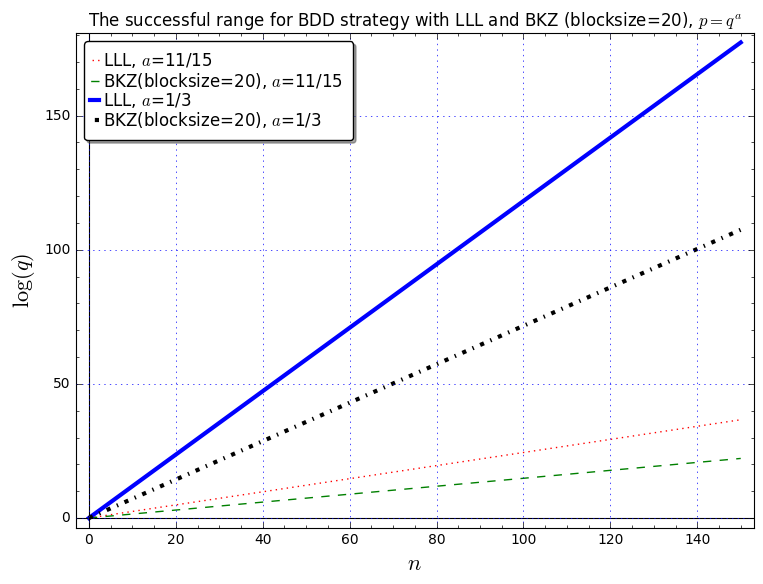
\includegraphics[scale=0.5, bb=0 0 560 430]{picture.png}
	\caption{We plot the graphs of the lines $\log (q_{\text{min}})=\lceil-4n  \log (c_{\mathcal{A}})/\alpha^2 \rceil$ corresponding to $\alpha=11/15$ and $\alpha=1/3$. For LLL, we use $c_{\text{LLL}}=0.9775$ and for BKZ of block size $20$ we use $c_{\text{BKZ}}=0.9868$.}
	\label{fig:success_range}
\end{figure}
%=======================
\subsubsection{Optimal Number of LWR Samples for BDD  Strategy.}
%=======================
The optimal number of LWR samples $m$ should be chosen such that the right hand side of
$2\sigma \leq c_{\mathcal{A}} ^{m} q^{\frac{m-n}{m}}$ is maximum.
So the optimal value of $m$ should be:
\begin{equation}\label{eq12} 
m=\left \lfloor \sqrt{\frac{n\log (q)}{- \log (c_{\mathcal{A}})}} \right\rceil.
\end{equation}
Remind that, the optimal number of samples typically  used in attacking LWE problems (e.g., see  \cite{LP11, MR09})  is
%\begin{equation}\label{eq123} 
$m=\left \lfloor \sqrt{\frac{n\log (q)}{ \log (\delta_{\mathcal{A}})}} \right\rceil,$
%\end{equation}
%====================
which along with \eqref{eq12} again convince us that $\delta_{\mathcal{A}} \approx 1/c_{\mathcal{A}}$ (see Subsection \ref{sec2.2}).

\section{Modulus Switching for BDD Strategy on LWR} \label{sec5}
%====================
 We will analyze the so-called $q'$-reduction which reduces an LWR$_{m,n,q,p}(\chi_s)$ instance to an LWE modulo $q'$ instance. Then we estimate the optimal $q'$ and an associated condition such that the BDD strategy on LWE modulo $q'$ instance is more efficient than the BDD strategy on LWE modulo $q$ instance. 

%=======================
\subsection{Reducing LWR$_{m,n,q,p}(\chi_s)$ to LWE Modulo $q'$}
%=======================

Let
$(\mathbf{a}, c=\left\lfloor \langle \mathbf{a},\mathbf{s} \rangle \right\rceil_{q,p}) \in \mathbb{Z}_q^{n} \times \mathbb{Z}_p$  be an LWR sample. We reduce this LWR sample to the LWE sample modulo $q'$ of the form $(\mathbf{a}',c'=\langle \mathbf{a}',\mathbf{s} \rangle+e') \in \mathbb{Z}_{q'}^{n} \times \mathbb{Z}_{q'}$ with
$
c'=\left \lfloor (q'/q) \cdot c \right \rceil
$ clarified below
where $\mathbf{a}'=\left\lfloor (q'/q)\cdot \mathbf{a} \right\rceil$. We call the error $e'$ $q'$-\textit{error}. We now take a closer look into the process of generating $e'$. Recall that,
$c=\lfloor \langle \mathbf{a}, \mathbf{s} \rangle \rceil_{q,p} =({p}/{q})\cdot \langle \mathbf{a}, \mathbf{s} \rangle+p\cdot u+e_1$
for some $u\in \mathbb{Z}$, where $e_1 \leftarrow \frac{1}{q}\cdot \mathcal{U} \left(T \right )$ with $T=\{-\lfloor q/2 \rfloor,...,\lfloor q/2 \rfloor \}$ (see \eqref{eq4} and the proof of Theorem 1).


Now with $q'$-reduction we will obtain
\begin{equation*}
c_2:=\frac{q'}{p}\cdot c=\left \langle \left \lfloor \frac{q'}{q}\mathbf{a} \right \rceil, \mathbf{s} \right\rangle +\left \langle \frac{q'}{q} \mathbf{a}-  \left \lfloor \frac{q'}{q} \mathbf{a}\right \rceil , \mathbf{s} \right\rangle +q'\cdot u+e_2,
\end{equation*}
where $e_2:=\frac{q'}{p}\cdot e_1 \leftarrow \frac{q'}{pq} \cdot  \mathcal{U}(T).$ Hence
\begin{equation*}
c':=\lfloor c_2 \rceil \text{ mod }q'=\left \langle \left \lfloor \frac{q'}{q}\mathbf{a} \right \rceil, \mathbf{s} \right\rangle \text{ mod }q' +\left \langle \frac{q'}{q} \mathbf{a}-  \left \lfloor \frac{q'}{q} \mathbf{a}\right \rceil , \mathbf{s} \right\rangle +e_2+e_3,
\end{equation*}
where $e_3 \in(-\frac{1}{2}, \frac{1}{2}].$ The $q'$-error is 
$e':=e_2+e_3+e_4,$
with $e_4:=\left \langle \frac{q'}{q} \mathbf{a}-  \left \lfloor \frac{q'}{q} \mathbf{a}\right \rceil , \mathbf{s} \right\rangle=\sum_{1}^{n}\left( \frac{q'}{q} a_i-  \left \lfloor \frac{q'}{q} a_i\right \rceil  \right)\cdot s_i$. 

\subsubsection{Distribution of $q'$-Error.} 
The behavior of $q'$-error is mainly affected by that of $e_2$ (following a uniform distribution (cf. Section \ref{sec3})) and $e_4$ (following a Gaussian distribution via Central Limit Theorem (cf. \cite[Lemma 2]{APS15})). Then, using the Equation  \eqref{keycon} on the convolution of two distributions, the probability density function of $e'$ can be approximated by
\begin{equation}\label{keypdf}
\begin{split}
f(y)&=\frac{p\sqrt{6}}{q'\sqrt{\pi n \sigma_s ^2}} \int_{-\frac{q'}{2p}}^{\frac{q'}{2p}}\exp\left(-\frac{6(x-y)^2}{n\sigma_s^2}\right)dx=\frac{p}{q'\sqrt{\pi}}\int_ {\frac{\sqrt{6} \left(-\frac{q'}{2p}-y \right)}{{\sqrt{n}\sigma_s}}}^ {\frac{\sqrt{6} \left(\frac{q'}{2p}-y \right)}{{\sqrt{n}\sigma_s}}} \exp(-\zeta^2)d\zeta\\
&=\frac{p}{2q'} \cdot \left[\mathrm{erf} \left( \frac{\sqrt{6} \left(\frac{q'}{2p}-y \right)}{\sqrt{n}\sigma_s} \right) +\mathrm{erf} \left( {\frac{\sqrt{6} \left(\frac{q'}{2p}+y \right)}{{\sqrt{n}\sigma_s}}} \right)\right].
\end{split}
\end{equation}
Its derivative is $$f'(y)=\frac{\sqrt{6}p}{2\sqrt{\pi n} q'\sigma_s} \cdot \left[-\text{exp} \left( \frac{-6 \left(\frac{q'}{2p}-y \right)^2}{n\sigma^2_s} \right) +\text{exp} \left( \frac{-6 \left(\frac{q'}{2p}+y \right)^2}{n\sigma^2_s} \right) \right].$$



The function $f(y)$ is symmetric through origin and it has convex bell-shaped curve reaching its highest value $h(q')=({p}/{q'}) \cdot \mathrm{erf} \left( (\sqrt{6}q')/(2p\sqrt{n}\sigma_s)\right)$ 
at $y=0$.
Note that the functions $f'(y)$ and $h(q')$ tend to 0 as $q'$ increases. Thus, if $q' \gg p$, the error $e'$ will tend to follow a uniform distribution. By contrast, when $q' \approx p$, the error $e'$ will tend to be distributed via a Gaussian distribution. 

The behavior of $q'$-error $e'$ is complex, therefore we cannot use \eqref{eq18} or \eqref{eqkk} to estimate the success probability of the BDD strategy in solving the LWE modulo $q'$. Also, on the other hand, we cannot compare the success probability of the BDD strategy on LWE modulo $q'$ with that on LWE modulo $q$ using the formulas \eqref{eq18} or \eqref{eqkk}. This is why we need to use Heuristic 1.
\subsubsection {Variance of $q'$-Error.}
We consider the variances of $e_2$, $e_3$ and $e_4$. The variance of $e_2$ will be
$\sigma_2^2:=\left({q'^2}/{(q^2p^2)}\right)\cdot \left(\left(\left(2\lfloor q/2 \rfloor+1 \right)^2-1\right)/{12}\right),$
the variance of $e_3$ is $\sigma_3^2=\frac{1}{12}$ . The variance $\sigma^2_4$ of $e_4$ can be approximated as sum of $n$ summands in which each summand is uniform on $[-\frac{1}{2}\sigma_s,\frac{1}{2}\sigma_s]$ where $\sigma_s$ is the variance of the secret $\mathbf{s}$. Hence  $\sigma^2_4=\frac{n}{12}\sigma^2_s.$
We assume that $e_2, e_3$ and $e_4$ are three independent random variables, then the variance of $e'$ is estimated by
\begin{equation}\label{eq13}
\sigma'^2 := \sigma_2^2+\sigma_3^2+\sigma_4^2\approx \frac{1}{12} \left(n\sigma^2_s+\frac{q'^2}{q^2p^2}\left(q^2+2q \right)+1 \right)=\frac{1}{12} \left(Mq'^2+N \right),
\end{equation}
where   $M:=(q^2+2q)/(p^2q^2)$ and $N:=n\sigma_s^2+1.$
%=======================
\subsection {Optimizing $q'$ for BDD Strategy}
%=======================

Assume that we have $m$ LWR samples each of which is a pair 
$(\mathbf{a}, c=\left\lfloor \langle \mathbf{a},\mathbf{s} \rangle \right\rceil_{q,p}) \in \mathbb{Z}_q^{n} \times \mathbb{Z}_p$. We reduce the LWR instance to:

\begin{itemize}
	\item The LWE modulo $q$  instance consists of $m$ LWE samples of the form $(\mathbf{a},c_1) \in \mathbb{Z}_q^{n} \times \mathbb{Z}_q$ where
$c_1 =\langle \mathbf{a}, \mathbf{s} \rangle \text{ mod } q+e$
where \textit{$q$-error} $e$ has variance of $ \sigma^2 \approx \frac{q^2+2qp}{12p^2}.$
We call this approach \textit{$q$-approach}.
 \item The LWE modulo $q'$ instance consists of $m$ LWE samples of the form $(\mathbf{a}',c') \in \mathbb{Z}_{q'}^{n} \times \mathbb{Z}_{q'}$
 where $c'=\langle \mathbf{a}',\mathbf{s} \rangle \text{ mod } q'+e'$ and $\mathbf{a}'=\left\lfloor ({q'}/{q}) \cdot \mathbf{a} \right\rceil,$ and the $q'$-error $e'$ has variance of  
 $
 \sigma'^2 \approx \frac{1}{12} \left(Mq'^2+N \right),
 $ with $M=(q^2+2q)/(p^2q^2)$ and $N=n\sigma_s^2+1.$
 We call this approach \textit{$q'$-approach}.
\end{itemize} 
For short, we say that the success probability of the BDD strategy in solving the LWE modulo $q$ instance (resp., the LWE modulo $q$ instance) as \textit{the success probability of the $q$-approach} (resp., the success probability of the $q'$-approach).
Notice that, in this section, the number of samples $m$ is arbitrary as long as $m > n$. However, $m$ will be optimally chosen via \eqref{eq12} in our experiments.


Our goal is to choose $q'$ such that the success probability of  the $q'$-approach is highest and certainly higher than that of the $q$-approach. The key idea is to use Heuristic 1. According to the heuristic, the success probability of the $q$-approach is
\begin{equation}\label{keyw}
\mathrm{Pr} \left[\frac{q^{m-n}}{\sigma^m} \geq  \frac{2^m}{c_{\mathcal{A}}^{m^2}}\right].
\end{equation}
Similarly, that of the $q'$-approach is
\begin{equation}\label{keya}
\mathrm{Pr} \left[\frac{q'^{m-n}}{\sigma'^m} \geq  \frac{2^m}{c_{\mathcal{A}}^{m^2}}\right].
\end{equation}

Set $P':=\frac{ q'^{m-n}}{ \sigma'^m} $ and $ P:= \frac{ q^{m-n}}{ \sigma^m}$. The Equations \eqref{keyw} and \eqref{keya} say that if $P' \geq P$ then the success probability of the $q'$-approach will be higher than that of the $q$-approach. Hence in order to achieve our goal, we can choose $q'$ such that $P' \geq P$ and
 \begin{equation}\label{eqn}
P' \text{ is maximum}.
\end{equation} 
The condition $P' \geq P$ is equivalent to
\begin{equation}\label{eqk1}
\frac{q'^{m-n}}{\sqrt{(Mq'^2+N)^m}} \geq \frac{q^{m-n}}{\sqrt{(\frac{q^2+2qp}{p^2})^m}}.
\end{equation}
The Equation \eqref{eqk1} can be rewritten as  
\begin{equation}\label{eqk2}
q'^{2(m-n)} \cdot (q^2+2qp)^m \geq q^{2(m-n)} \cdot p^{2m} \cdot (Mq'^2+N)^m.
\end{equation}

Now, it is the time to state the main theorem of this section.
\subsubsection{Theorem 2.} \label{theorem3} 
(i) \textit{The optimal choice for $q'$ satisfying \eqref{eqn} is}
\begin{equation} \label{eq26}
q' \approx \sqrt{\frac{(m-n)(n\sigma_s^2+1)p^2q^2}{n(q^2+2q)}}.
\end{equation}

(ii) \textit{The sufficient condition under which the $q'$-approach has success probability higher than that of the $q$-approach is that 
	\begin{equation}\label{key6}
	(n\sigma_s^2+1)p^2 \leq q^2+2q.
	\end{equation}}
	 %In other words, the sufficient condition is that
%$q'^{\text{opt}} \leq \sqrt{\frac{m-n}{n}}\cdot q$.}
\proof Set $M:=(q^2+2q)/(p^2q^2)$ and $N:=n\sigma_s^2+1$ as in \eqref{eq13}.

For (i),  we have $P'=\frac{ q'^{m-n}}{ \sigma'^m}=\frac{q'^{m-n}\sqrt{12^m}}{\sqrt{(Mq'^2+N)^m}}$. Define $t:={q'}^2$, then ${P'}^2=\frac{t^{m-n}12^m}{(Mt+N)^m}$. It is easy to see that $t_0:=\frac{(m-n)N}{nM}$ maximizes ${P'}^2$. So we should choose $q' \approx \sqrt{t_0}= \sqrt{\frac{(m-n)N}{nM}}$.
 
 For (ii), by plugging $q'^2=t_0$ into \eqref{eqk2} and after some calculations, we get
 \begin{equation}\label{key1}
[(m-n)N]^{m-n} \cdot  (q^2+2qp)^m \cdot  n^n \geq q^{2(m-n)} \cdot p^{2m} \cdot (mN)^m \cdot  M^{m-n}.
 \end{equation}
 Now taking the natural logarithm on \eqref{key1} we have 
  \begin{equation*}
  \begin{split}
 &(m-n)\ln (m-n)+ (m-n)\ln (N) +m \ln (q^2+2qp)+ n \ln (n) \\
 &\geq 2(m-n)\ln (q)+  2m \ln(p)+ m \ln(m)+ m\ln(N) +(m-n)\ln(M).
 \end{split}
 \end{equation*}
 Using the facts that 
 $m \ln (q^2+2qp) \geq m\ln (q^2+2q),$ 
 and that 
 $(m-n)\ln (m-n)+ n \ln(n) \geq m \ln(m)$
 \footnote[3]{It is easy to check that the funtion $x\ln(x)$ is concave  over $(0, +\infty)$.} along with some simple calculations, we imply the sufficient condition for \eqref{eqk2} to hold is that $ \ln(N)+[\ln(p^2)-\ln (q^2+2q)]\leq 0$
which is equivalent to
$$ (n\sigma_s^2+1)p^2 \leq q^2+2q.$$
 \qed
 
 
  %=======================
 \begin{remark} 
 %=======================
 The Equation \eqref{eq26} looks like the same as the Equation \eqref{keye}. The main difference between them is that the Equation  \eqref{eq26} gets involved with the number of samples $m$. This suggests that in order to apply the modulus switching technique for the BDD strategy on LWE, one should find the new $q'$ rather than using the one in \eqref{keye}.
  \end{remark} 


   %=======================
 \begin{remark} 
 	%=======================
 Recall that, if \eqref{key6} holds then so does the \eqref{eqk2}, hence \eqref{eqk1} also holds. Thus the gap \begin{equation}\label{gap}
 \mathtt{GAP}:=(q^2+2q)-(n\sigma_s^2+1)p^2
 \end{equation}
  can be used to estimate the gap between two approaches. Obviously, the bigger the gap $\mathtt{GAP}$ is, the better the $q'$-approach is in comparison with the $q$-approach. The Equation \eqref{gap} yields that: (i) the $q'$-approach is more suitable for short secret LWR instances which have $\sigma_s$ small; (ii) in the case that $p$ close to $q$, i.e.,  $\alpha \approx 1$,  the $q'$-approach is not more efficient than the $q$-approach and (iii) by contrast, in the case $p$ is much smaller than $q$, i.e.,  $\alpha \ll 1$, the $q'$-approach is much more efficient than the $q$-approach. 
 \end{remark} 

   %=======================
 \begin{remark} 
 	%=======================
By Remark 1, given $\alpha$, if $n$ increases then $\log (q_{\text{min}})$ also increases. This is likely to make the gap $\mathtt{GAP}$ increase. We can see this trend from the columns entitled ``$\mathtt{GAP}$ \eqref{gap}" in the Tables 2-5. 
\end{remark} 


	
%======================
\section{Implementation and Experimental Results} \label{sec6}
%======================
We implemented the BDD strategy on LWR problem to evaluate the efficacy of the $q'$-approach in comparison with the $q$-approach. In our experiments, we used SageMath version 8.1 \cite{Sag81} to implement the BDD strategy. The LBR algorithm used in our experiments is LLL \cite{LLL82}. We used the the function``.LLL()"  to call the floating point implementation of LLL in the \textit{fplll} library which is included in SageMath with the default reduction parameter $0.99$. By using such an LLL algorithm, we have the corresponding constant mentioned in \eqref{eq1} is $c_{\text{LLL}}=0.9775$ (see Section \ref{sec2.2}). 
%We used mainly a Macbook Pro (Retina, 13-inch, Early 2015) with Intel Iris Graphics 6100 1536 MB 2.7 GHz Intel Core i5  and memory of 8 GB 1867 MHz DDR3.


\begin{table}[pt]
	\centering
	\small\addtolength{\tabcolsep}{1.5pt}
	\caption{\textbf{How to proceed with our experiments?} } 
	
	\begin{tabular}{p{10cm}}
		
		\hline
		\hline
		
		1. First, choose $\alpha$, then choose $n$ and compute $\log (q_{\text{min}})$ by \eqref{eq11}. \\
		2. Next, choose $\log (q)$ to be around $\log (q_{\text{min}})$, from which we have $q$ and $p$. After that we compute $q'$ by \eqref{eq26} and compute $m$ by \eqref{eq12}.\\
		3. For each tuple ($\alpha, n, q_{\text{min}}, q, p, q'$), sample 10 LWR instances or 5 LWR instances up to $\alpha$ and $n$. (For $\alpha=11/15$, we sample 10 LWR instances. For the rest of $\alpha$'s, we sample 5 LWR instances.)\\
		4. For each LWR instance, transform it to LWE modulo $q$ and LWE modulo $q'$. \\
		5. Finally, run BDD attack on these two LWE instances. \\
		\hline
		\hline
		
	\end{tabular}
	\label{table:1}
\end{table}

We introduce some parameters and notations presented in our experimental results: $\alpha$ is the bit ratio of $p$ and $q$, i.e., $\alpha=\log (p)/ \log (q)$; $n$ is the dimension of secret; $\log (q_{\text{min}})$ is the smallest bit size of $q$ computed by \eqref{eq11} given $\alpha$, $n$; $\log (q')$, $\log (q)$, $\log(p)$ are the bit size of modulo $q'$ computed by \eqref{eq26}, of moduli $q$ and $p$, respectively; $m$ is the optimal number of LWR samples for BDD attack computed by \eqref{eq12} (we use the same number of samples $m$ in both the $q$-approach and $q'$- approach); the columns entitled ``$\mathtt{GAP}$", ``succ($q$)", ``succ($q'$)" ,  ``rHF($q$)" and ``rHF($q'$)" represent the size of the gap $\mathtt{GAP}$ in \eqref{gap}, the success probability of the $q$-approach and of the $q'$-approach, the rHF of the $q$-approach and of the $q'$-approach, respectively. Note that, rHF($q$) and rHF($q'$) are computed using the formula \eqref{eq1}.
%=======================



\begin{table}[pt]
	\caption{\textbf{Compare $q' $-approach with the $q$-approach $(\alpha=11/15)$} } 
	\centering
	\small\addtolength{\tabcolsep}{0.8pt}
	
	\begin{tabular}{| c|c | c | c | c | c | c | c |c|c| }
		\hline
		\hline
		$(n, \log (q_{\text{min}}))$& $\log (q)$ & $\log (p)$  & $\log (q')$ & $\  m\ $  &$\mathtt{GAP}$& succ($q$) & succ($q'$)&rHF$(q)$&rHF$(q')$\\
		\hline
		\hline
		
		\parbox[t]{13mm}{\multirow{2}{*}{(60,15)}}&\textbf{15}&11&\textbf{14}&166&9.5776e8&\textbf{0\%}&\textbf{60\%}&1.0202&1.0200\\
		
		&\textbf{17}&12&\textbf{15}&176&1.6716e10&100\%&100\%&1.0203&1.0197\\
		\hline
	
	\parbox[t]{13mm}{\multirow{4}{*}{(80,20)}}&\textbf{17}&12&\textbf{15}&204&1.6567e10&0\%&0\%&1.0209&1.0200\\
		
			&\textbf{18}&13&\textbf{16}&209&6.6267e10&\textbf{20\%}&\textbf{80\%}&1.0205&1.0200\\
		
		&\textbf{20}&15&\textbf{19}&221&1.0603e12&\textbf{80\%}&\textbf{100\%}&1.0209&1.0200\\
		
		&\textbf{22}&16&\textbf{20}&232&1.7435e13&100\%&100\%&1.0205&1.0200\\
		
		\hline

		\parbox[t]{13mm}{\multirow{2}{*}{(100,25)}}&\textbf{20}&15&\textbf{19}&247&1.0507e12&\textbf{20\%}&\textbf{60\%}&1.0210&1.0203\\
		
		
		&\textbf{25}&18&\textbf{22}&276&1.1228e15&100\%&100\%&1.0212&1.0195\\
		
		
		
		
		\hline
	\end{tabular}
	\label{table:2}
	%\end{table}
	
	
	%begin{table}
	\caption{\textbf{Compare the $q'$-approach with the $q$-approach $(\alpha=2/3)$} } 
	\centering
	\begin{tabular}{| c|c | c | c | c | c | c | c |c|c| }
		\hline
		\hline
		
		$(n, \log (q_{\text{min}}))$& $\log (q)$ & $\log (p)$  & $\log (q')$ & $m$  &$\mathtt{GAP}$& succ($q$) & succ($q'$)&rHF$(q)$&rHF$(q')$\\
		
		
		\hline
		\hline
		
		\parbox[t]{13mm}{\multirow{3}{*}{(60,18)}}&\textbf{16}&11&\textbf{14}&171&4.1791e9&80\%&80\%&1.0203& 1.0199\\	
		
		
		
		&\textbf{17}&11&\textbf{14}&176&1.7064e10&\textbf{20\%}&\textbf{60\% }&1.0201&1.0188\\	
		&\textbf{18}&12&\textbf{15}&181&6.8256e10&\textbf{100\%}&\textbf{100\% }&1.0202&1.0191\\		
		\hline
		\parbox[t]{13mm}{\multirow{2}{*}{(80,24)}}&\textbf{21}&14&\textbf{18}&226&4.3882e12&\textbf{20\%}&\textbf{100\%}&1.0203&1.0187\\	
		&\textbf{23}&15&\textbf{19}&237&7.0330e13&\textbf{40\%}&\textbf{100\% }&1.0215&1.0180\\	
			&\textbf{24}&16&\textbf{20}&242&2.8132e14&\textbf{100\%}&\textbf{100\% }&1.0208&1.0183\\		
		
		
		\hline
		\parbox[t]{13mm}{\multirow{3}{*}{(100,30)}}&\textbf{24}&16&\textbf{20}&270&2.8128e14&\textbf{0\%}&\textbf{80\% }&1.0211&1.0184\\
		
		&\textbf{26}&17&\textbf{21}&281&4.5028e15&\textbf{0\%}&\textbf{100\% }&1.0211&1.0179\\
		&\textbf{28}&19&\textbf{23}&292&7.2045e16&100\%&100\% &1.0213&1.0182\\	
		
		\hline	
	\end{tabular}
	\label{table:3}
	
	\caption{\textbf{Compare the $q'$-approach with the $q$-approach $(\alpha=1/2)$} } 
	\centering
	\begin{tabular}{| c | c | c | c | c | c | c | c | c| c|}
		
		\hline
		\hline
		$(n, \log (q_{\text{min}}))$& $\log (q)$ & $\log (p)$  & $\log (q')$ & $m$  &$\mathtt{GAP}$& succ($q$) & succ($q'$)&rHF$(q)$&rHF$(q')$\\
		\hline
		\hline
		\parbox[t]{13mm}{\multirow{2}{*}{(60,32)}}&\textbf{26}&13&\textbf{17}&218&4.5036e15&\textbf{0\%}&\textbf{100\%}&1.0210&1.0142 \\			
		&\textbf{30}&15&\textbf{19}&234&1.1529e18&\textbf{20\%}&\textbf{100\%} &1.0201&1.0140\\	
		\hline 
			\parbox[t]{13mm}{\multirow{2}{*}{(80,43)}}	&\textbf{27}&17&\textbf{21}&256&1.8014e16&\textbf{0\%}&\textbf{80\% }&1.0208&1.0146\\
			&\textbf{35}&18&\textbf{22}&292&1.1806e21&\textbf{0\%}&\textbf{100\% }&1.0209&1.0140\\
		\hline
			%&\textbf{26}&13&\textbf{17}&281&4.5036e15&0\%&0\% &1.0209&1.0143\\
			\parbox[t]{13mm}{\multirow{2}{*}{(100,53)}}&\textbf{31}&16&\textbf{20}&307&4.5036e15&\textbf{0\%}&\textbf{60\%} &1.0214&1.0143\\
			&\textbf{37}&19&\textbf{23}&336&1.8889e22&\textbf{0\%}&\textbf{100\%} &1.0213&1.0138\\		
		\hline
		
	\end{tabular}
	\label{table:4}
	
	
	\caption{\textbf{Compare the $q'$-approach with the $q$-approach $(\alpha=1/3)$}}  
	\centering
	\begin{tabular}{| c | c | c | c | c | c | c | c | c| c|}
		
		\hline
		\hline
		$(n, \log (q_{\text{min}}))$& $\log (q)$ & $\log (p)$  & $\log (q')$ & $m$  &$\mathtt{GAP}$& succ($q$) & succ($q'$)&rHF$(q)$&rHF$(q')$\\	
		\hline
		\hline
		\parbox[t]{13mm}{\multirow{1}{*}{(40,48)}}&\textbf{38}	&13&\textbf{17}&215&7.5558e22&\textbf{0\%}&\textbf{100\%}&1.0212&1.0096\\
		%&\textbf{48}&16&\textbf{20}&242&7.9228e28&N/A&\textbf{100\% }\\
		
		\hline
	
	\parbox[t]{13mm}{\multirow{1}{*}{(60,71)}}	&\textbf{49}&16&\textbf{20}&299&3.1691e29&\textbf{0\%}&\textbf{100\% }&1.0215&1.0091\\	
		\hline
		\parbox[t]{13mm}{\multirow{1}{*}{(80,95)}}&\textbf{61}&20&\textbf{24}&386&5.3169e36&\textbf{0\%}&\textbf{100\% }&1.0214&1.0088\\		
		\hline
	\parbox[t]{13mm}{\multirow{1}{*}{(100,119)}}&\textbf{59}&20&\textbf{24}&424&3.3231e35&\textbf{0\%}&\textbf{100\% }&1.0213&1.0091\\	

		\hline	
	\end{tabular}
	\label{table:5}
\end{table}


The experimental results are summarized in the Tables 2 - 5 each of which corresponds to one value $\alpha$.
The small secret $\mathbf{s}$ is drawn uniformly at random over $\{-1,0,1\}^n$. The first $\alpha=11/15$ is inspired from choosing parameters in the work of \cite{BBGM+17}, the last one $\alpha=1/3$ comes from  \cite{DTV15} whilst two middle ones $\alpha=2/3$ and $\alpha=1/2$ are additionally suggested by us. 
We refer to Table 1 for generating parameters, sampling LWR instances, as well as running BDD attack on the corresponding LWE instances.

We highlight some noticeable things from our experimental results:
\begin{itemize}
	\item In all cases, the rHF of the $q$-approach is always bigger than that of the $q'$-approach. Interestingly, the rHF of the $q'$-approach becomes smaller once $\alpha$ declines while the rHF of the $q$-approach does not seem to change, namely, rHF$(q') \approx 1.0201$ for all considered $\alpha$'s. Recall that, smaller root Hermite factor means that the LWE modluo $q'$ instance is more easily solved by BDD strategy than the LWE modluo $q$ instance (see Section \ref{heu}).
	\item When $\alpha$ is close to $1$, such as $\alpha=11/15$, the $q'$-approach does not outweigh the $q$-approach much (see Table \ref{table:2}). In constrast, when $\alpha$ is closer to 0 than 1, e.g., $\alpha=1/3$,  $q'$ approach is much efficient than the $q$-approach in terms of success probability, rHF and even running time (although we do not add the runtime data in the tables due to lacking of space) since $q'$ is quite close to $p$ (see Table \ref{table:5}). For example, with $\alpha=1/3, n=100$, we $\log (q')=59$ that is much less than $\log (q)=119$.
	\item The bit size $\log(q')$ is quite close to $\log(p)$. Namely, in all considered cases, we have $\log(q')-\log(p)$ equals to $3$ \text{ or } $4$. It seems that the difference $\log(q')-\log(p)$ increases (but slowly) once either $n$ increases or/and $\alpha$ decreases.   
	\item With fixed $\alpha$, the successful range for BDD strategy seems to be widen when $n$ grows. For instance, consider $\alpha=11/15$:  in case $n=60$ we have $\log({q_{\text{min}}})=15$, if choose $\log (q)=15$ then succ($q$)=0\%; by contrast, with $n=80$, we have $\log({q_{\text{min}}})=20$, hence if $\log (q)=20$ then succ($q$)=80\%. Similarly, for $n=100$, $\log({q_{\text{min}}})=25$ then succ($q$)=100\% with if $\log (q)=25$.

\item With fixed $\alpha$, it seems that when $n$ grows the difference succ$(q')-$succ$(q)$ between two approaches also increases. Take $\alpha=2/3$ for example, we can compare the  difference succ$(q')-$succ$(q)$ for $n=60$ with the difference succ$(q')-$succ$(q)$ for respect to $n=100$ (see Table \ref{table:3}). This suggests that for large $n$, $q'$-approach actually outweighs $q$-approach.

\item Also, fixed $\alpha$ and $n$, the difference succ$(q')-$succ$(q)$ seems to depend on choosing $q$ around $q_{\text{min}}$. If $q$ is much less than $q_{\text{min}}$ then both succ$(q)$ and succ($q'$) are $0\%$. For example, for $\alpha=11/15, n=80$, we have $\log({q_{\text{min}}})=20$, if we choose $\log (q)=17$ then $\log (q')=15$ and succ($q$)=succ($q'$)=0\%. However, for the case  $q$ is sufficiently bigger than $q_{\text{min}}$, the success probability of two approaches is 1. Certainly, in that case, depending on which one is smaller (typically, $q'$ is smaller than $q$), we choose the corresponding approach to reduce the running time of BDD attack. 
\item Remarkably, when $\alpha$ is close to $0$ (e.g., $\alpha=1/3$), the $q'$-approach significantly widens the successful range. For instance, with $\alpha=1/3$, $n=80$ and $\log({q_{\text{min}}})=95$, if we choose $\log(q)=61$, then $\log(q')=24$ and succ($q$)=0\% but succ($q'$)=100\% (see Table \ref{table:5}).
\end{itemize}
The experimental phenomena listed above can be theoretically explained by our theoretical results. Our experimental results, in turn, also strongly support our reasonings. From our experiments, we can conclude that for LWR-based cryptosystems, one should choose two moduli $q$ and $p$ that are not so far from each other. 

%===============
\section{Conclusion}
%===============

In this paper, we concentrated on applying the idea of the modulus switching technique for solving LWR instances. To do that, we scrutinized the behavior of LWR errors in order to evaluate their variances more precisely. Furthermore, the successful range in which a search LWR instance can be solved by the BDD strategy associated with Babai's Nearest Plane algorithm was also determined. Based on the successful range, we take LWR instances that are consistent with our experiments. Experimental results support our theoretical result that applying modulus switching technique for the BDD strategy on (small secret) search-LWR$_{m,n,q,p}(\chi_s)$ will be very efficient, especially if the bit ratio $\log(p)/\log(q)$ is close to 0 and/or $n$ is sufficiently large. While our experiments were just proceeded with toy examples in which $n$ is quite small, we believe that our modulus switching approach still performs very well for large $n$'s used in practice. 

Although our work does not give any warning to current LWR-based cryptosystems, it suggests that the modulus switching technique should be carefully considered in security analyses of prospective LWR-based (maybe even LWE-based) cryptosystems due to its remarkable effects. Considering effects of the modulus switching on other attacking strategies against LWR problem (even LWE) and analyzing its runtime effectiveness are our future works.  

\subsubsection{Acknowledgments.} This work was supported by JST CREST Grant Number JPMJCR14D6, Japan. This work was also supported by JSPS KAKENHI Grant Number 16H02830.
We would like to thank the anonymous reviewers for their careful reading as well as very helpful comments and suggestions.
\medskip

\bibliographystyle{splncs04}    %{abbrv}%{splncs04}
\bibliography{ref}




\end{document}